
            \documentclass[tikz]{standalone}
            \begin{document}
            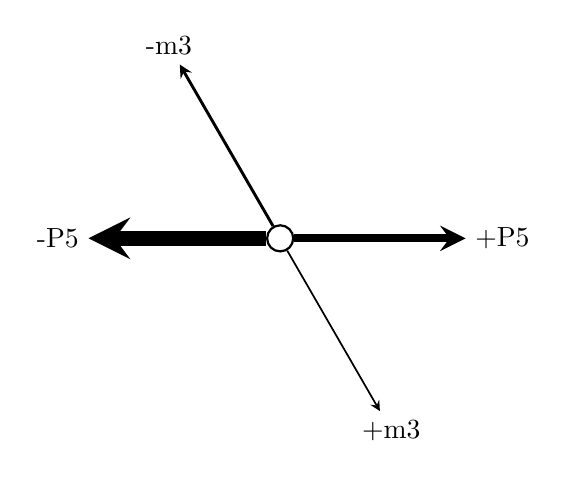
\begin{tikzpicture}[scale=3.5, ->, >=stealth]

            % the circle
            \node (origin) at (0,0) [draw,circle,black,fill=white,thick]{};
            % constant scaling for widths
            \def\cons{10}
            
                    \node (0) at +(0*360/6:0.8066976934682587) {+P5};
                    \path (origin) edge [line width=\cons*0.2944063219439405] node {} (0);
                    
                    \node (1) at +(-1*360/6:0.8066976934682587) {+m3};
                    \path (origin) edge [line width=\cons*0.0619583004309872] node {} (1);
                    
                    \node (3) at +(-3*360/6:0.8066976934682587) {-P5};
                    \path (origin) edge [line width=\cons*0.5384056467574481] node {} (3);
                    
                    \node (4) at +(-4*360/6:0.8066976934682587) {-m3};
                    \path (origin) edge [line width=\cons*0.10522973086762404] node {} (4);
                    
            \end{tikzpicture}
            \end{document}
            